\begin{appendices}
  \addtocontents{toc}{\protect\setcounter{tocdepth}{1}}
    \makeatletter
    \addtocontents{toc}{%
      \begingroup
      \let\protect\l@chapter\protect\l@section
      \let\protect\l@section\protect\l@subsection
    }
    \makeatother

    \chapter{User Manual}
      This document is also available online: \\ http://bit.ly/points\_extraction\_user\_manual

\noindent\hrulefill

\noindent This guide will list steps to complete the analysis for a single arbitrary discussion. The only software that you need to install on your computer is Docker and Docker Compose. Docker hosts lightweight virtual machines called containers that run each of our services.

\section{Installation}
\begin{enumerate}
	\item{\href{https://docs.docker.com/engine/installation/}{Install Docker} and the \href{https://docs.docker.com/compose/install/}{Docker Compose interface}. This varies depending on the host operating system.}
	\item{Check that you can run \texttt{docker ps} and see output starting: \texttt{CONTAINER ID...}}
	\item{Change directory into the project folder \texttt{cd {project-folder-path}}}
	\item{Run \texttt{docker-compose build}, this will download all the dependencies for each of the project's services. This includes a series of operating system images and the CoreNLP framework and will take some time (allow 20-25 mins on a 20mbps connection, time also depends on the resources allocated to Docker).}
\end{enumerate}

\section{Setting Up a Corpus}
\begin{enumerate}
	\item{First you need to get a corpus in place to run the analysis on. This guide will talk you through using the Abortion corpus we used. Download the corpus to the \texttt{analysis\_api} folder: \\  \texttt{curl -L http://bit.ly/1QxG9i7 > analysis\_api/abortion.zip}}
	\item{Now unzip the downloaded corpus: \\ \texttt{unzip analysis\_api/abortion.zip -d analysis\_api/abortion \&\& \\ mv analysis\_api/abortion/**/* analysis\_api/abortion/ \&\& \\ rm -r analysis\_api/abortion/5*}}
	\item{(OPTIONAL) Inspect a corpus file: \texttt{cat analysis\_api/abortion/post\_1}. Lines like \texttt{\#key=value} are parsed into metadata. These are optional.}
	\item{It is now time to start a console in the \texttt{analysis\_api} service. To do this run: \texttt{docker-compose run analysis\_api /bin/bash}.}
	\item{You will now have a new prompt \texttt{/app\#}. The current directory is \texttt{analysis\_api}, file changes are synced between this container and the host. Type \texttt{ls} and you will see the contents of the \texttt{analysis\_api} folder.}
	\item{Before extracting points from the corpus we need to clean the posts for invalid characters and parse any metadata. Run \texttt{ruby clean.rb abortion} to do this for all of the files in the raw abortion corpus we downloaded.}
\end{enumerate}

\section{Extracting Points}
\begin{enumerate}
	\item{You are now ready to extract a list of points from the corpus. To do this run \texttt{ruby collector.rb abortion}. This will take around 10-15 mins and is quite an intensive task. Output is written to \texttt{abortion\_points.txt} in the \texttt{analysis\_api} directory. This will be a large file (approx. 50mb), The first line is a list of topics and the following lines represent each point in JSON.}
	\item{When you have finished running the points extraction process you  can exit the analysis\_api console with \texttt{exit}.}
\end{enumerate}

\section{Cleaning/Curating Points}
\begin{enumerate}
	\item{To prepare the list of points for use in summarization they must first be reformatted. First you need to move your extracted points file into the \texttt{curator} directory. From the project root run: \\ \texttt{mv analysis\_api/abortion\_points.txt curator/abortion\_points.txt}}
	\item{From the project root directory run \texttt{docker-compose run curator /bin/bash} to get a console ready to run the curation task.}
	\item{To clean the list for summarization run: \\ \texttt{go run main.go abortion\_points.txt > abortion\_points\_clean.txt}}
\end{enumerate}

\section{Generating Summaries}
\begin{enumerate}
	\item{First get a clean list of points to use in generating the summary. From the project root run: \\ \texttt{mv curator/abortion\_points\_clean.txt summarizer/abortion\_points\_clean.txt}.}
	\item{Now run: \texttt{docker-compose run summarizer /bin/bash} to get a console prepared for generating summaries.}
	\item{To generate a summary for your clean list of points run: \texttt{ruby summarizer.rb abortion\_points\_clean.txt}}
	\item{This will save a file in the \texttt{summarizer} directory called \texttt{abortion\_formatted.html}. This is the end result and should be viewed in a browser.}
\end{enumerate}




    \chapter{Maintenance Manual\label{app:maintain}}
      \section{First section}
      \section{Second section}

    \chapter{Discussion Graph Representation\label{app:disc_graph}}
      \begin{figure}[h]
        \centering
        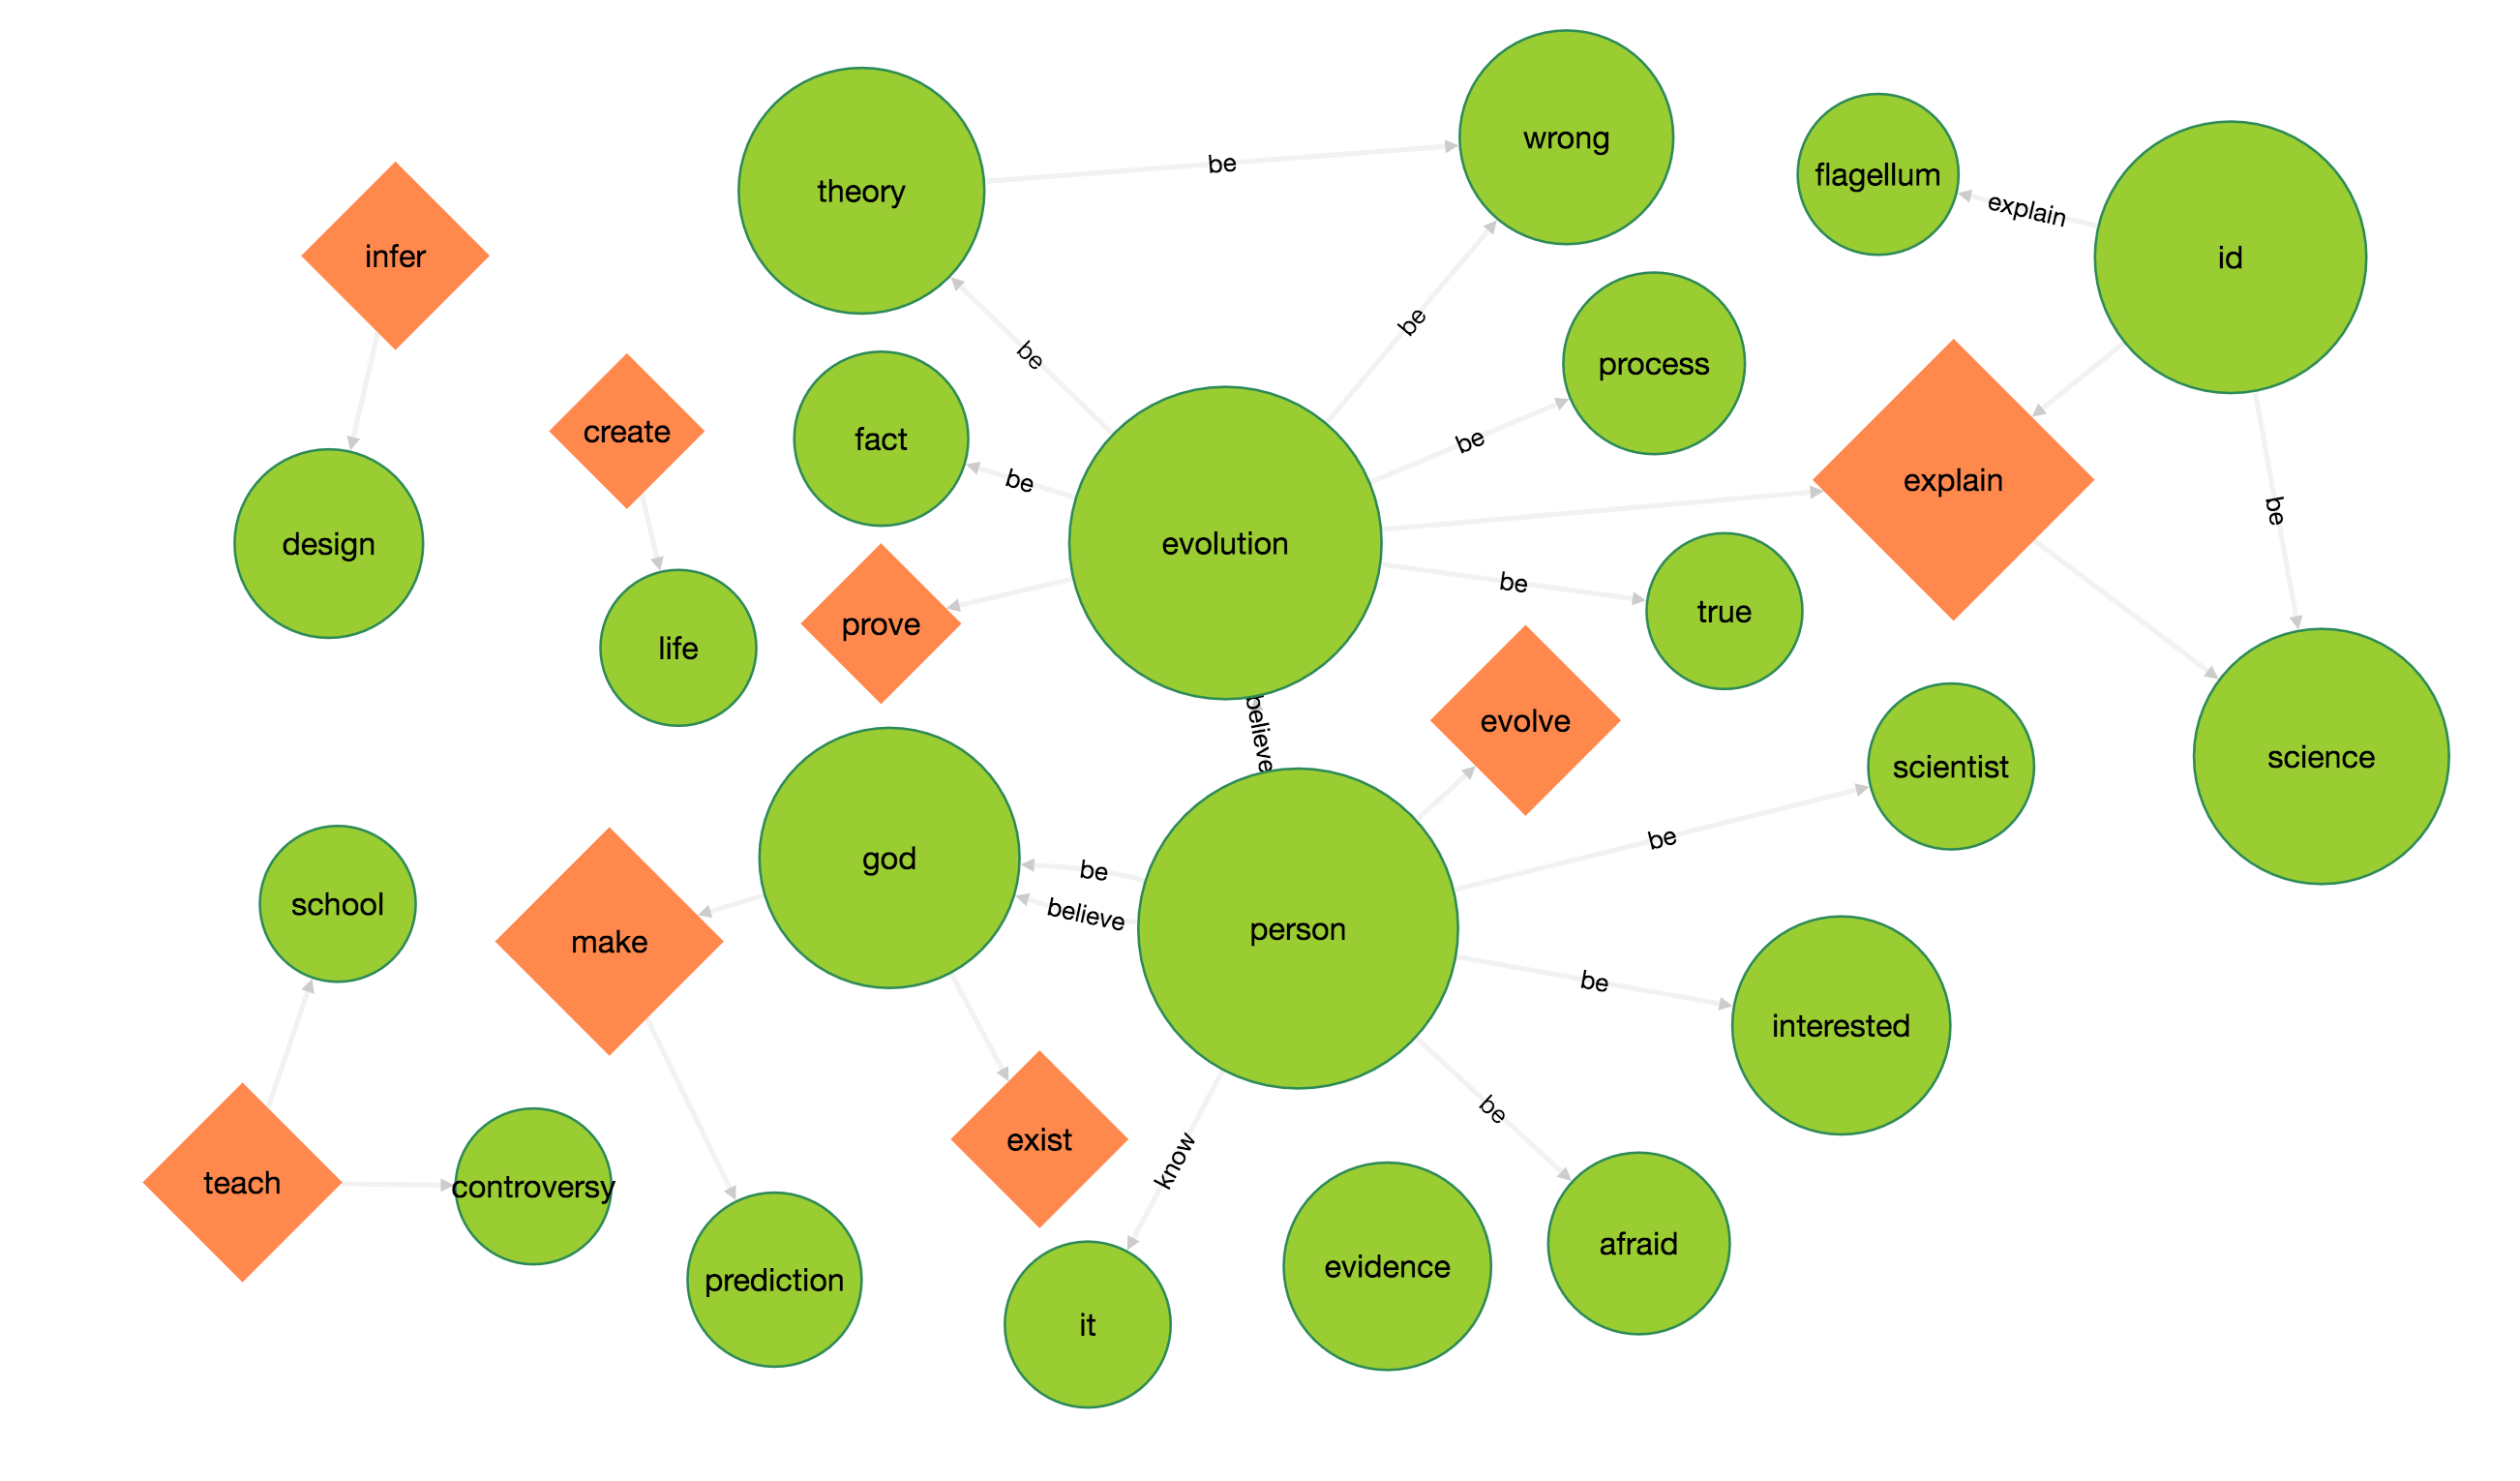
\includegraphics[width=0.8\textwidth]{disc_graph}
        \caption{A sample graph representation of the abortion discussion}
      \end{figure}

    \chapter{Blacklists\label{app:blacklists}}
      \section{Ambiguous subjects}
        \textit{it, that, this, which, what}

      \section{Disallowed Person Actions}
        The following verbs are not allowed in a 2 component point with a \texttt{PERSON.nsubj}:

        \textit{agree, argue, ask, begin, believe, believe, call, care, change, close, come, come, continue, debate, disagree, end, explain, fail, feel, feel, find, follow, get, go, go, guess, happen, hear, leave, live, lose, make, move, object, open, read, realize, refer, show, sit, speak, stand, start, support, take, talk, tell, think, try, understand, wonder, write}

      \section{Disallowed Points}
        \texttt{PERSON.nsubj be.verb} cannot be completed by: \textit{able, aware, correct, false, favor, glad, good, here, interested, likely, one, right, say, sorry, sure, true, willing, wrong}

        \noindent\texttt{PERSON.nsubj want.verb} cannot be completed by: \textit{have, what, what do}

        \noindent\texttt{PERSON.nsubj} cannot be completed by: \textit{say.verb what.dobj, mean.verb what.dobj, know.verb what.dobj, believe.verb what.dobj, see.verb what.dobj, see.verb argument.dobj, have.verb problem.dobj, tell.verb they.dobj, think.verb what.dobj, argue.verb in.prep fact.dobj, argue.verb with.prep you.dobj}

        \begin{itemize}
		  \item{debate.nsubj be.verb about.dobj}
		  \item{question.nsubj be.verb}
		  \item{make.verb claim.dobj}
		  \item{ask.verb yourself.dobj}
		  \item{thing.nsubj happen.verb}
		  \item{something.nsubj happen.verb}
        \end{itemize}

    \chapter{Evaluation Questionnaire Structure \label{app:evaluation-questionnaire-layouts}}
      \TBox[fill=red!15]{13cm}{
        \large Study 1 Questionnaire ($\times$6 variations in Latin Square) \\
        \normalsize
        \TBox[fill=black!1]{12.7cm}{
          \textbf{Section 1} Plain vs. Stock (see Appendix \ref{app:survey-section}) \\
          \small Order switches (3$\times$ Plain/Stock, 3$\times$ Stock/Plain)
          \normalsize

          \TBox[fill=white]{6cm}{
            Plain Summary (Topic A)
          }
          \TBox[fill=white]{6cm}{
            Stock Summary (Topic A)
          }
          \TBoxDash[fill=black!15]{12.4cm}{
            \textit{4 factor ratings; overall rating \& free text comment}
          }
        }
        \TBox[fill=black!1]{12.7cm}{
          \textbf{Section 2} Layout vs. Stock \\
          \small Order switches (3$\times$ Layout/Stock, 3$\times$ Stock/Layout)
          \normalsize

          \TBox[fill=white]{6cm}{
            Layout Summary (Topic \textbf{B})
          }
          \TBox[fill=white]{6cm}{
            Stock Summary (Topic \textbf{B})
          }
          \TBoxDash[fill=black!15]{12.4cm}{
            \textit{4 factor ratings; overall rating \& free text comment}
          }
        }
        \TBox[fill=black!1]{12.7cm}{
          \textbf{Section 3} Layout vs. Formatted \\
          \small Order switches (3$\times$ Layout/Formatted, 3$\times$ Form./Lay.)

          \small Summaries share content, only differ in formatting

          \small Layout summary reused from Section 2
          \normalsize

          \TBox[fill=white]{6cm}{
            Layout Summary (Topic \textbf{B})
          }
          \TBox[fill=white]{6cm}{
            Formatted Summ. (Topic \textbf{B})
          }
          \TBoxDash[fill=black!15]{12.4cm}{
            \textit{Overall rating only \& free text comment}
          }
        }
      }

      \vspace{2mm}
      \noindent\TBox[fill=green!15]{13cm}{
        \large Study 2 Questionnaire ($\times$6 variations) \\
        \normalsize
        \TBox[fill=black!1]{12.7cm}{
          \textbf{Section 1} Rating Extracts \\
          \normalsize

          \TBox[fill=white]{12.4cm}{
            Extract Set (Topic A) \textbf{($\times$3)} (see Appendix \ref{app:extract-survey-section})\\
            \TBoxDash[fill=black!15]{12.1cm}{
              \textit{Rating 1/5 per extract (approx. 10 extracts)}
            }
          }
        }
        \TBox[fill=black!1]{12.7cm}{
          \textbf{Section 2} Bigram vs. Random \\

          \TBox[fill=white]{6cm}{
            Bigram Summary (Topic A)
          }
          \TBox[fill=white]{6cm}{
            Random Summary (Topic A)
          }
          \TBoxDash[fill=black!15]{12.4cm}{
            \textit{Overall rating only \& free text comment}
          }
        }
      }

      \vspace{2mm}
      \noindent\TBox[fill=blue!15]{13cm}{
        \large Study 3 Questionnaire ($\times$2 variations each, $\times$6 variations total) \\
        \normalsize
        Participants had \textbf{two sheets}, each with different topics.
        \TBox[fill=black!1]{12.7cm}{
          \textbf{Section 1} Layout vs. Stock \\

          \TBox[fill=white]{6cm}{
            Layout Summary (Topic A)
          }
          \TBox[fill=white]{6cm}{
            Stock Summary (Topic A)
          }
          \TBoxDash[fill=black!15]{12.4cm}{
            \textit{Free text comments only}
          }
        }
      }

    \chapter{Summary Comparison Survey Section\label{app:survey-section}}
      \begin{figure}[h]
        \caption{An example study 1 survey section comparing a plain and stock survey.}
        \centering
        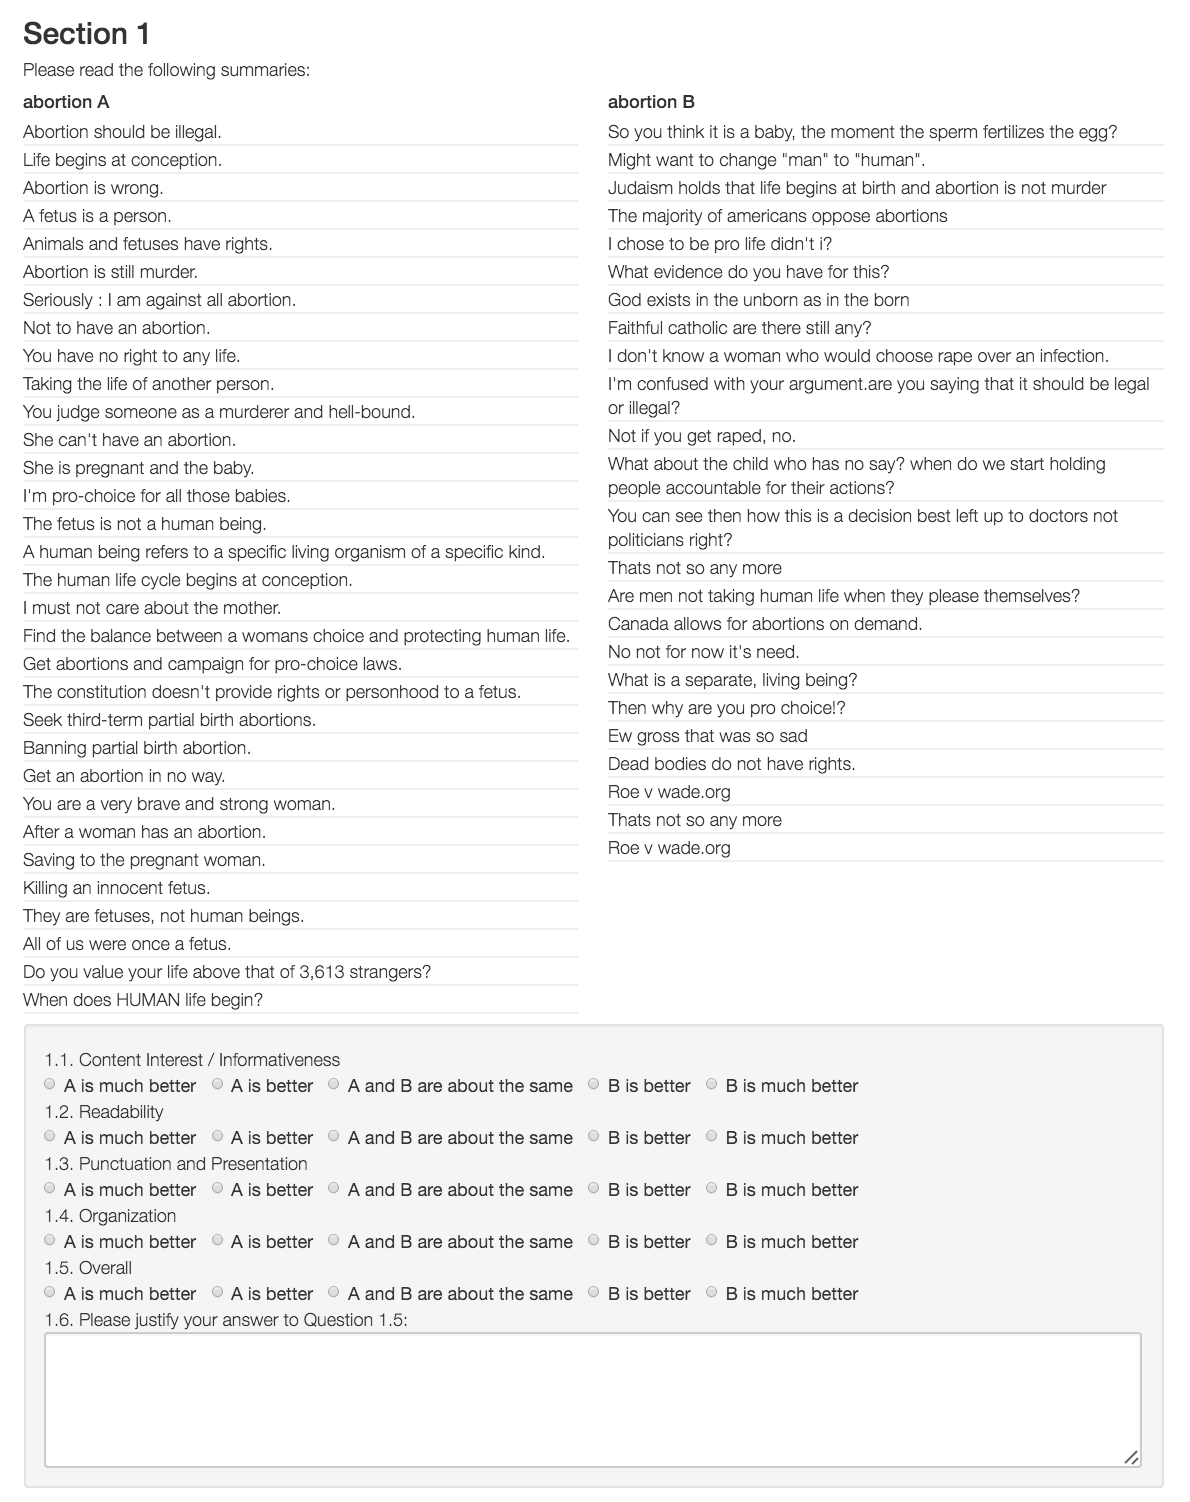
\includegraphics[width=0.9\textwidth]{survey}
      \end{figure}

    \chapter{Extract Survey Section\label{app:extract-survey-section}}
      \begin{figure}[h]
        \caption{An example study 2 survey section where participants rated extracts.}
        \centering
        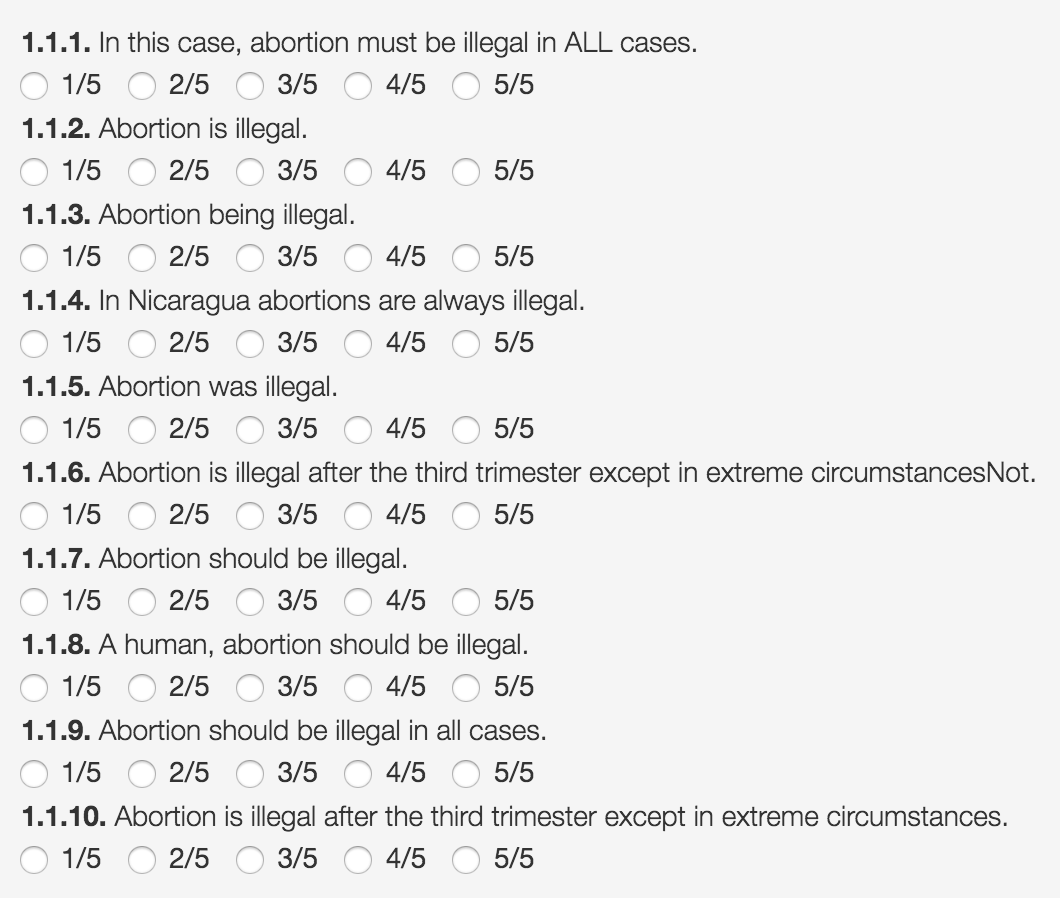
\includegraphics[width=0.9\textwidth]{survey2}
      \end{figure}

  \addtocontents{toc}{\endgroup}
\end{appendices}
